\documentclass[12pt]{exam}
\usepackage{amsthm}
\usepackage{libertine}
\usepackage[utf8]{inputenc}
\usepackage[margin=1in]{geometry}
\usepackage{amsmath,amssymb}
\usepackage{multicol}
\usepackage[shortlabels]{enumitem}
\usepackage{siunitx}
\usepackage{cancel}
\usepackage{graphicx}
\usepackage{pgfplots}
\usepackage{listings}
\usepackage{tikz}



\pgfplotsset{width=10cm,compat=1.9}
\usepgfplotslibrary{external}
\tikzexternalize

\newcommand{\class}{Math 101-002} % This is the name of the course 
\newcommand{\examnum}{Quiz 4} % This is the name of the assignment
\newcommand{\examdate}{April 3} % This is the due date





\begin{document}
\pagestyle{plain}
\thispagestyle{empty}

\noindent
\textbf{\class}\\
\textbf{\examnum}, \textbf{\examdate} \\

% Name \hfill CSU ID \# \hspace{2.25in}

%\vspace{10 pt}

\setlength{\tabcolsep}{3.5cm} % Default value: 6pt
\renewcommand{\arraystretch}{1.5}
\setlength\extrarowheight{1cm}
\begin{tabular}{ |c|c| } 
 \hline
 Name   & CSU ID \#  \\ 
 \hline
\end{tabular}
% ---
\vspace{10pt}

Be sure to read each question fully and carefully. Even if you don't know the answer please take this opportunity to reflect on what you may need to practice for the exam.


\begin{enumerate} 

    \item Consider the following weighted graph $G$:
    \begin{figure}[h]
        \centering


\tikzset{every picture/.style={line width=0.75pt}} %set default line width to 0.75pt        

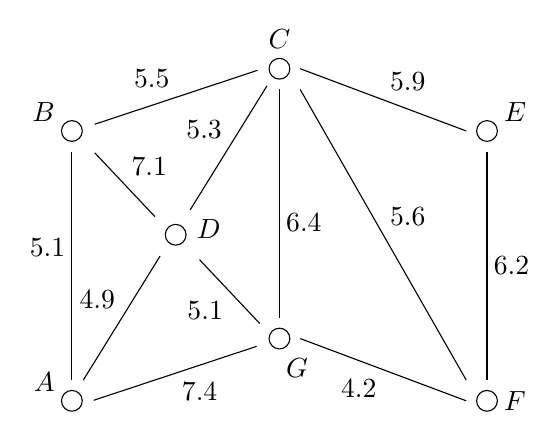
\begin{tikzpicture}[x=0.75pt,y=0.75pt,yscale=-1,xscale=1]
%uncomment if require: \path (0,300); %set diagram left start at 0, and has height of 300

%Shape: Circle [id:dp05512682112725742] 
\draw   (100,105) .. controls (100,102.24) and (102.24,100) .. (105,100) .. controls (107.76,100) and (110,102.24) .. (110,105) .. controls (110,107.76) and (107.76,110) .. (105,110) .. controls (102.24,110) and (100,107.76) .. (100,105) -- cycle ;
%Shape: Circle [id:dp37072597810767505] 
\draw   (200,75) .. controls (200,72.24) and (202.24,70) .. (205,70) .. controls (207.76,70) and (210,72.24) .. (210,75) .. controls (210,77.76) and (207.76,80) .. (205,80) .. controls (202.24,80) and (200,77.76) .. (200,75) -- cycle ;
%Shape: Circle [id:dp3763549497766574] 
\draw   (100,235) .. controls (100,232.24) and (102.24,230) .. (105,230) .. controls (107.76,230) and (110,232.24) .. (110,235) .. controls (110,237.76) and (107.76,240) .. (105,240) .. controls (102.24,240) and (100,237.76) .. (100,235) -- cycle ;
%Shape: Circle [id:dp8983000317077905] 
\draw   (200,205) .. controls (200,202.24) and (202.24,200) .. (205,200) .. controls (207.76,200) and (210,202.24) .. (210,205) .. controls (210,207.76) and (207.76,210) .. (205,210) .. controls (202.24,210) and (200,207.76) .. (200,205) -- cycle ;
%Shape: Circle [id:dp19038098852300678] 
\draw   (150,155) .. controls (150,152.24) and (152.24,150) .. (155,150) .. controls (157.76,150) and (160,152.24) .. (160,155) .. controls (160,157.76) and (157.76,160) .. (155,160) .. controls (152.24,160) and (150,157.76) .. (150,155) -- cycle ;
%Straight Lines [id:da17692309627353553] 
\draw    (199,83.25) -- (162,143) ;
%Straight Lines [id:da32795803599293327] 
\draw    (147.5,165.25) -- (110.5,225) ;
%Straight Lines [id:da9321494854298098] 
\draw    (116,115.5) -- (145,146.25) ;
%Straight Lines [id:da6788470123675919] 
\draw    (166.5,167) -- (195.5,197.75) ;
%Straight Lines [id:da6081990495255584] 
\draw    (116,101.75) -- (194.5,75.75) ;
%Straight Lines [id:da7068537454160456] 
\draw    (115.5,234.75) -- (194,208.75) ;
%Straight Lines [id:da033903285827347696] 
\draw    (105,115) -- (105,225) ;
%Straight Lines [id:da21385775272897756] 
\draw    (205,85) -- (205,195) ;
%Shape: Circle [id:dp7839742417573956] 
\draw   (300,105) .. controls (300,102.24) and (302.24,100) .. (305,100) .. controls (307.76,100) and (310,102.24) .. (310,105) .. controls (310,107.76) and (307.76,110) .. (305,110) .. controls (302.24,110) and (300,107.76) .. (300,105) -- cycle ;
%Shape: Circle [id:dp32979392250331063] 
\draw   (300,235) .. controls (300,232.24) and (302.24,230) .. (305,230) .. controls (307.76,230) and (310,232.24) .. (310,235) .. controls (310,237.76) and (307.76,240) .. (305,240) .. controls (302.24,240) and (300,237.76) .. (300,235) -- cycle ;
%Straight Lines [id:da7139419536553874] 
\draw    (305,115) -- (305,225) ;
%Straight Lines [id:da7117674674918515] 
\draw    (215,75) -- (295,105) ;
%Straight Lines [id:da33204635137335015] 
\draw    (215,205) -- (295,235) ;
%Straight Lines [id:da5247863294102606] 
\draw    (215,85) -- (295,225) ;

% Text Node
\draw (98,231.6) node [anchor=south east] [inner sep=0.75pt]    {$A$};
% Text Node
\draw (98,101.6) node [anchor=south east] [inner sep=0.75pt]    {$B$};
% Text Node
\draw (205,66.6) node [anchor=south] [inner sep=0.75pt]    {$C$};
% Text Node
\draw (164,146.4) node [anchor=north west][inner sep=0.75pt]    {$D$};
% Text Node
\draw (312,101.6) node [anchor=south west] [inner sep=0.75pt]    {$E$};
% Text Node
\draw (312,235) node [anchor=west] [inner sep=0.75pt]    {$F$};
% Text Node
\draw (207,213.4) node [anchor=north west][inner sep=0.75pt]    {$G$};
% Text Node
\draw (179,185.77) node [anchor=north east] [inner sep=0.75pt]    {$5.1$};
% Text Node
\draw (153.25,85.35) node [anchor=south east] [inner sep=0.75pt]    {$5.5$};
% Text Node
\draw (127,191.73) node [anchor=south east] [inner sep=0.75pt]    {$4.9$};
% Text Node
\draw (132.5,127.48) node [anchor=south west] [inner sep=0.75pt]    {$7.1$};
% Text Node
\draw (178.5,109.73) node [anchor=south east] [inner sep=0.75pt]    {$5.3$};
% Text Node
\draw (103,166.6) node [anchor=south east] [inner sep=0.75pt]    {$5.1$};
% Text Node
\draw (156.75,225.15) node [anchor=north west][inner sep=0.75pt]    {$7.4$};
% Text Node
\draw (207,143.4) node [anchor=north west][inner sep=0.75pt]    {$6.4$};
% Text Node
\draw (257,86.6) node [anchor=south west] [inner sep=0.75pt]    {$5.9$};
% Text Node
\draw (257,151.6) node [anchor=south west] [inner sep=0.75pt]    {$5.6$};
% Text Node
\draw (307,170) node [anchor=west] [inner sep=0.75pt]    {$6.2$};
% Text Node
\draw (253,223.4) node [anchor=north east] [inner sep=0.75pt]    {$4.2$};


\end{tikzpicture}

    \end{figure}
    \begin{enumerate}
    \item How many edges make up a spanning tree of $G$?
    \item What is the redundancy of $G$?
    \item Use Kruskal's algorithm to find an minimum-weight spanning tree of $G$. Draw the corresponding tree in the following space.
    \end{enumerate}
    \vfill
\newpage
    \item Consider the following directed graph specifying the precedence order for the tasks $A$ through $H$:
    \begin{figure}[h]
        \centering


\tikzset{every picture/.style={line width=0.75pt}} %set default line width to 0.75pt        

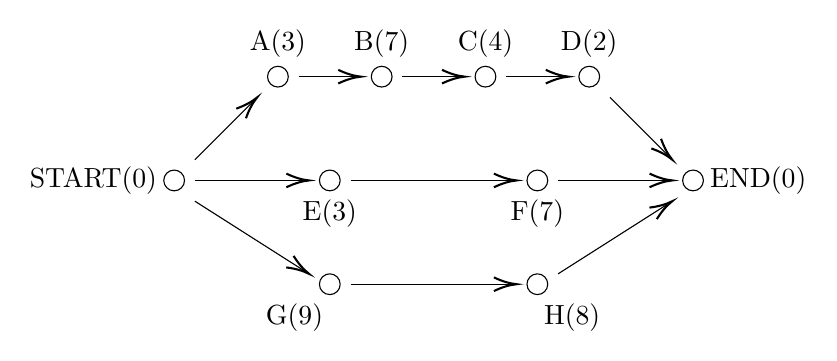
\begin{tikzpicture}[x=0.75pt,y=0.75pt,yscale=-1,xscale=1]
%uncomment if require: \path (0,300); %set diagram left start at 0, and has height of 300

%Shape: Circle [id:dp3806789383117838] 
\draw   (100,105) .. controls (100,102.24) and (102.24,100) .. (105,100) .. controls (107.76,100) and (110,102.24) .. (110,105) .. controls (110,107.76) and (107.76,110) .. (105,110) .. controls (102.24,110) and (100,107.76) .. (100,105) -- cycle ;
%Shape: Circle [id:dp36494538661860054] 
\draw   (200,55) .. controls (200,52.24) and (202.24,50) .. (205,50) .. controls (207.76,50) and (210,52.24) .. (210,55) .. controls (210,57.76) and (207.76,60) .. (205,60) .. controls (202.24,60) and (200,57.76) .. (200,55) -- cycle ;
%Shape: Circle [id:dp6499160923199319] 
\draw   (150,55) .. controls (150,52.24) and (152.24,50) .. (155,50) .. controls (157.76,50) and (160,52.24) .. (160,55) .. controls (160,57.76) and (157.76,60) .. (155,60) .. controls (152.24,60) and (150,57.76) .. (150,55) -- cycle ;
%Shape: Circle [id:dp899995398586803] 
\draw   (300,55) .. controls (300,52.24) and (302.24,50) .. (305,50) .. controls (307.76,50) and (310,52.24) .. (310,55) .. controls (310,57.76) and (307.76,60) .. (305,60) .. controls (302.24,60) and (300,57.76) .. (300,55) -- cycle ;
%Shape: Circle [id:dp5265204886981469] 
\draw   (250,55) .. controls (250,52.24) and (252.24,50) .. (255,50) .. controls (257.76,50) and (260,52.24) .. (260,55) .. controls (260,57.76) and (257.76,60) .. (255,60) .. controls (252.24,60) and (250,57.76) .. (250,55) -- cycle ;
%Shape: Circle [id:dp482939064607797] 
\draw   (175,105) .. controls (175,102.24) and (177.24,100) .. (180,100) .. controls (182.76,100) and (185,102.24) .. (185,105) .. controls (185,107.76) and (182.76,110) .. (180,110) .. controls (177.24,110) and (175,107.76) .. (175,105) -- cycle ;
%Shape: Circle [id:dp5774999245991583] 
\draw   (275,105) .. controls (275,102.24) and (277.24,100) .. (280,100) .. controls (282.76,100) and (285,102.24) .. (285,105) .. controls (285,107.76) and (282.76,110) .. (280,110) .. controls (277.24,110) and (275,107.76) .. (275,105) -- cycle ;
%Shape: Circle [id:dp027740632068865345] 
\draw   (175,155) .. controls (175,152.24) and (177.24,150) .. (180,150) .. controls (182.76,150) and (185,152.24) .. (185,155) .. controls (185,157.76) and (182.76,160) .. (180,160) .. controls (177.24,160) and (175,157.76) .. (175,155) -- cycle ;
%Shape: Circle [id:dp638076700175927] 
\draw   (275,155) .. controls (275,152.24) and (277.24,150) .. (280,150) .. controls (282.76,150) and (285,152.24) .. (285,155) .. controls (285,157.76) and (282.76,160) .. (280,160) .. controls (277.24,160) and (275,157.76) .. (275,155) -- cycle ;
%Shape: Circle [id:dp6043863899206905] 
\draw   (350,105) .. controls (350,102.24) and (352.24,100) .. (355,100) .. controls (357.76,100) and (360,102.24) .. (360,105) .. controls (360,107.76) and (357.76,110) .. (355,110) .. controls (352.24,110) and (350,107.76) .. (350,105) -- cycle ;
%Straight Lines [id:da46938004765128616] 
\draw    (115,95) -- (143.59,66.41) ;
\draw [shift={(145,65)}, rotate = 135] [color={rgb, 255:red, 0; green, 0; blue, 0 }  ][line width=0.75]    (10.93,-3.29) .. controls (6.95,-1.4) and (3.31,-0.3) .. (0,0) .. controls (3.31,0.3) and (6.95,1.4) .. (10.93,3.29)   ;
%Straight Lines [id:da7935095531650652] 
\draw    (115,105) -- (168,105) ;
\draw [shift={(170,105)}, rotate = 180] [color={rgb, 255:red, 0; green, 0; blue, 0 }  ][line width=0.75]    (10.93,-3.29) .. controls (6.95,-1.4) and (3.31,-0.3) .. (0,0) .. controls (3.31,0.3) and (6.95,1.4) .. (10.93,3.29)   ;
%Straight Lines [id:da5280838564210045] 
\draw    (115,115) -- (168.31,148.93) ;
\draw [shift={(170,150)}, rotate = 212.47] [color={rgb, 255:red, 0; green, 0; blue, 0 }  ][line width=0.75]    (10.93,-3.29) .. controls (6.95,-1.4) and (3.31,-0.3) .. (0,0) .. controls (3.31,0.3) and (6.95,1.4) .. (10.93,3.29)   ;
%Straight Lines [id:da3278551571524768] 
\draw    (190,105) -- (268,105) ;
\draw [shift={(270,105)}, rotate = 180] [color={rgb, 255:red, 0; green, 0; blue, 0 }  ][line width=0.75]    (10.93,-3.29) .. controls (6.95,-1.4) and (3.31,-0.3) .. (0,0) .. controls (3.31,0.3) and (6.95,1.4) .. (10.93,3.29)   ;
%Straight Lines [id:da5505828654107574] 
\draw    (290,105) -- (343,105) ;
\draw [shift={(345,105)}, rotate = 180] [color={rgb, 255:red, 0; green, 0; blue, 0 }  ][line width=0.75]    (10.93,-3.29) .. controls (6.95,-1.4) and (3.31,-0.3) .. (0,0) .. controls (3.31,0.3) and (6.95,1.4) .. (10.93,3.29)   ;
%Straight Lines [id:da38212929677952523] 
\draw    (165,55) -- (193,55) ;
\draw [shift={(195,55)}, rotate = 180] [color={rgb, 255:red, 0; green, 0; blue, 0 }  ][line width=0.75]    (10.93,-3.29) .. controls (6.95,-1.4) and (3.31,-0.3) .. (0,0) .. controls (3.31,0.3) and (6.95,1.4) .. (10.93,3.29)   ;
%Straight Lines [id:da026131803323604097] 
\draw    (215,55) -- (243,55) ;
\draw [shift={(245,55)}, rotate = 180] [color={rgb, 255:red, 0; green, 0; blue, 0 }  ][line width=0.75]    (10.93,-3.29) .. controls (6.95,-1.4) and (3.31,-0.3) .. (0,0) .. controls (3.31,0.3) and (6.95,1.4) .. (10.93,3.29)   ;
%Straight Lines [id:da05316480776786581] 
\draw    (265,55) -- (293,55) ;
\draw [shift={(295,55)}, rotate = 180] [color={rgb, 255:red, 0; green, 0; blue, 0 }  ][line width=0.75]    (10.93,-3.29) .. controls (6.95,-1.4) and (3.31,-0.3) .. (0,0) .. controls (3.31,0.3) and (6.95,1.4) .. (10.93,3.29)   ;
%Straight Lines [id:da90926798247493] 
\draw    (315,65) -- (343.59,93.59) ;
\draw [shift={(345,95)}, rotate = 225] [color={rgb, 255:red, 0; green, 0; blue, 0 }  ][line width=0.75]    (10.93,-3.29) .. controls (6.95,-1.4) and (3.31,-0.3) .. (0,0) .. controls (3.31,0.3) and (6.95,1.4) .. (10.93,3.29)   ;
%Straight Lines [id:da19940752405421558] 
\draw    (190,155) -- (268,155) ;
\draw [shift={(270,155)}, rotate = 180] [color={rgb, 255:red, 0; green, 0; blue, 0 }  ][line width=0.75]    (10.93,-3.29) .. controls (6.95,-1.4) and (3.31,-0.3) .. (0,0) .. controls (3.31,0.3) and (6.95,1.4) .. (10.93,3.29)   ;
%Straight Lines [id:da7166610433150618] 
\draw    (290,150) -- (343.31,116.07) ;
\draw [shift={(345,115)}, rotate = 147.53] [color={rgb, 255:red, 0; green, 0; blue, 0 }  ][line width=0.75]    (10.93,-3.29) .. controls (6.95,-1.4) and (3.31,-0.3) .. (0,0) .. controls (3.31,0.3) and (6.95,1.4) .. (10.93,3.29)   ;

% Text Node
\draw (98,105) node [anchor=east] [inner sep=0.75pt]   [align=left] {START(0)};
% Text Node
\draw (155,47) node [anchor=south] [inner sep=0.75pt]   [align=left] {A(3)};
% Text Node
\draw (205,47) node [anchor=south] [inner sep=0.75pt]   [align=left] {B(7)};
% Text Node
\draw (255,47) node [anchor=south] [inner sep=0.75pt]   [align=left] {C(4)};
% Text Node
\draw (305,47) node [anchor=south] [inner sep=0.75pt]   [align=left] {D(2)};
% Text Node
\draw (180,113) node [anchor=north] [inner sep=0.75pt]   [align=left] {E(3)};
% Text Node
\draw (280,113) node [anchor=north] [inner sep=0.75pt]   [align=left] {F(7)};
% Text Node
\draw (178,163) node [anchor=north east] [inner sep=0.75pt]   [align=left] {G(9)};
% Text Node
\draw (282,163) node [anchor=north west][inner sep=0.75pt]   [align=left] {H(8)};
% Text Node
\draw (362,105) node [anchor=west] [inner sep=0.75pt]   [align=left] {END(0)};


\end{tikzpicture}
    \end{figure}\\
    If the priority list for the tasks is
    $$A,B,E,F,G,C,D,H,$$
    fill out a working schedule for two processors based on this:
\begin{figure}[h]
    \centering


\tikzset{every picture/.style={line width=0.75pt}} %set default line width to 0.75pt        

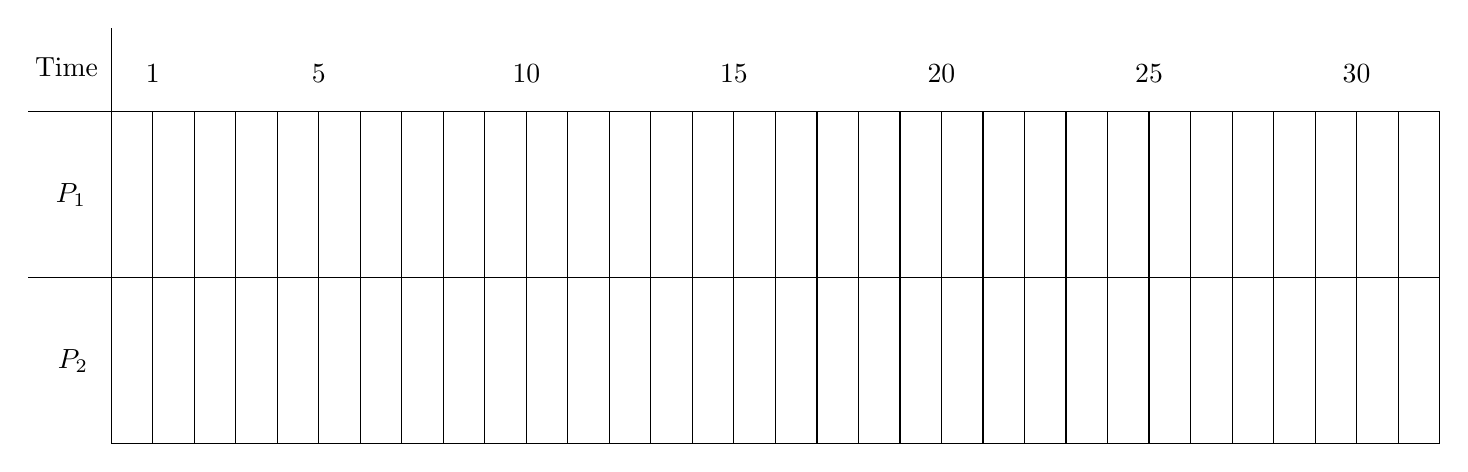
\begin{tikzpicture}[x=0.75pt,y=0.75pt,yscale=-1,xscale=1]
%uncomment if require: \path (0,300); %set diagram left start at 0, and has height of 300

%Shape: Rectangle [id:dp24634191044811404] 
\draw   (100,100) -- (120,100) -- (120,180) -- (100,180) -- cycle ;
%Shape: Rectangle [id:dp0429659201456678] 
\draw   (100,180) -- (120,180) -- (120,260) -- (100,260) -- cycle ;
%Shape: Rectangle [id:dp724185568085094] 
\draw   (120,100) -- (140,100) -- (140,180) -- (120,180) -- cycle ;
%Shape: Rectangle [id:dp1971394686075344] 
\draw   (120,180) -- (140,180) -- (140,260) -- (120,260) -- cycle ;

%Shape: Rectangle [id:dp14208471222022934] 
\draw   (140,100) -- (160,100) -- (160,180) -- (140,180) -- cycle ;
%Shape: Rectangle [id:dp5181649833827067] 
\draw   (140,180) -- (160,180) -- (160,260) -- (140,260) -- cycle ;
%Shape: Rectangle [id:dp024705872818378882] 
\draw   (160,100) -- (180,100) -- (180,180) -- (160,180) -- cycle ;
%Shape: Rectangle [id:dp6593215111016265] 
\draw   (160,180) -- (180,180) -- (180,260) -- (160,260) -- cycle ;


%Shape: Rectangle [id:dp5601104412265263] 
\draw   (180,100) -- (200,100) -- (200,180) -- (180,180) -- cycle ;
%Shape: Rectangle [id:dp6243674030023654] 
\draw   (180,180) -- (200,180) -- (200,260) -- (180,260) -- cycle ;
%Shape: Rectangle [id:dp361572737319631] 
\draw   (200,100) -- (220,100) -- (220,180) -- (200,180) -- cycle ;
%Shape: Rectangle [id:dp38072607731990515] 
\draw   (200,180) -- (220,180) -- (220,260) -- (200,260) -- cycle ;

%Shape: Rectangle [id:dp24410111025588388] 
\draw   (220,100) -- (240,100) -- (240,180) -- (220,180) -- cycle ;
%Shape: Rectangle [id:dp9289487874823138] 
\draw   (220,180) -- (240,180) -- (240,260) -- (220,260) -- cycle ;
%Shape: Rectangle [id:dp1675531973805633] 
\draw   (240,100) -- (260,100) -- (260,180) -- (240,180) -- cycle ;
%Shape: Rectangle [id:dp42842736509381496] 
\draw   (240,180) -- (260,180) -- (260,260) -- (240,260) -- cycle ;



%Shape: Rectangle [id:dp570712049630778] 
\draw   (260,100) -- (280,100) -- (280,180) -- (260,180) -- cycle ;
%Shape: Rectangle [id:dp2466523727768315] 
\draw   (260,180) -- (280,180) -- (280,260) -- (260,260) -- cycle ;
%Shape: Rectangle [id:dp5060320699058115] 
\draw   (280,100) -- (300,100) -- (300,180) -- (280,180) -- cycle ;
%Shape: Rectangle [id:dp1689347853879687] 
\draw   (280,180) -- (300,180) -- (300,260) -- (280,260) -- cycle ;

%Shape: Rectangle [id:dp4507595734329406] 
\draw   (300,100) -- (320,100) -- (320,180) -- (300,180) -- cycle ;
%Shape: Rectangle [id:dp982534237983468] 
\draw   (300,180) -- (320,180) -- (320,260) -- (300,260) -- cycle ;
%Shape: Rectangle [id:dp1631678051143246] 
\draw   (320,100) -- (340,100) -- (340,180) -- (320,180) -- cycle ;
%Shape: Rectangle [id:dp5944194617086641] 
\draw   (320,180) -- (340,180) -- (340,260) -- (320,260) -- cycle ;


%Shape: Rectangle [id:dp4506696475588067] 
\draw   (340,100) -- (360,100) -- (360,180) -- (340,180) -- cycle ;
%Shape: Rectangle [id:dp5251163959276807] 
\draw   (340,180) -- (360,180) -- (360,260) -- (340,260) -- cycle ;
%Shape: Rectangle [id:dp8970121753532935] 
\draw   (360,100) -- (380,100) -- (380,180) -- (360,180) -- cycle ;
%Shape: Rectangle [id:dp09604120050928688] 
\draw   (360,180) -- (380,180) -- (380,260) -- (360,260) -- cycle ;

%Shape: Rectangle [id:dp6786461877374534] 
\draw   (380,100) -- (400,100) -- (400,180) -- (380,180) -- cycle ;
%Shape: Rectangle [id:dp2857226586826398] 
\draw   (380,180) -- (400,180) -- (400,260) -- (380,260) -- cycle ;
%Shape: Rectangle [id:dp5118155589201975] 
\draw   (400,100) -- (420,100) -- (420,180) -- (400,180) -- cycle ;
%Shape: Rectangle [id:dp02332055995891058] 
\draw   (400,180) -- (420,180) -- (420,260) -- (400,260) -- cycle ;




%Shape: Rectangle [id:dp09201786735986228] 
\draw   (420,100) -- (440,100) -- (440,180) -- (420,180) -- cycle ;
%Shape: Rectangle [id:dp4512051015384675] 
\draw   (420,180) -- (440,180) -- (440,260) -- (420,260) -- cycle ;
%Shape: Rectangle [id:dp6888799892355403] 
\draw   (440,100) -- (460,100) -- (460,180) -- (440,180) -- cycle ;
%Shape: Rectangle [id:dp5408322391195265] 
\draw   (440,180) -- (460,180) -- (460,260) -- (440,260) -- cycle ;

%Shape: Rectangle [id:dp9240487360613258] 
\draw   (460,100) -- (480,100) -- (480,180) -- (460,180) -- cycle ;
%Shape: Rectangle [id:dp7907047176293046] 
\draw   (460,180) -- (480,180) -- (480,260) -- (460,260) -- cycle ;
%Shape: Rectangle [id:dp7711993665150441] 
\draw   (480,100) -- (500,100) -- (500,180) -- (480,180) -- cycle ;
%Shape: Rectangle [id:dp0794439433522377] 
\draw   (480,180) -- (500,180) -- (500,260) -- (480,260) -- cycle ;


%Shape: Rectangle [id:dp7133577773765207] 
\draw   (500,100) -- (520,100) -- (520,180) -- (500,180) -- cycle ;
%Shape: Rectangle [id:dp5709428535825334] 
\draw   (500,180) -- (520,180) -- (520,260) -- (500,260) -- cycle ;
%Shape: Rectangle [id:dp048091860857121915] 
\draw   (520,100) -- (540,100) -- (540,180) -- (520,180) -- cycle ;
%Shape: Rectangle [id:dp29806954262817353] 
\draw   (520,180) -- (540,180) -- (540,260) -- (520,260) -- cycle ;

%Shape: Rectangle [id:dp7362304160187053] 
\draw   (540,100) -- (560,100) -- (560,180) -- (540,180) -- cycle ;
%Shape: Rectangle [id:dp31715638418575287] 
\draw   (540,180) -- (560,180) -- (560,260) -- (540,260) -- cycle ;
%Shape: Rectangle [id:dp19180292773802454] 
\draw   (560,100) -- (580,100) -- (580,180) -- (560,180) -- cycle ;
%Shape: Rectangle [id:dp013153975221408376] 
\draw   (560,180) -- (580,180) -- (580,260) -- (560,260) -- cycle ;



%Shape: Rectangle [id:dp2560855508672938] 
\draw   (580,100) -- (600,100) -- (600,180) -- (580,180) -- cycle ;
%Shape: Rectangle [id:dp10848012493558179] 
\draw   (580,180) -- (600,180) -- (600,260) -- (580,260) -- cycle ;
%Shape: Rectangle [id:dp5891495301347475] 
\draw   (600,100) -- (620,100) -- (620,180) -- (600,180) -- cycle ;
%Shape: Rectangle [id:dp4335261678084191] 
\draw   (600,180) -- (620,180) -- (620,260) -- (600,260) -- cycle ;

%Shape: Rectangle [id:dp4232615059379129] 
\draw   (620,100) -- (640,100) -- (640,180) -- (620,180) -- cycle ;
%Shape: Rectangle [id:dp460576089660765] 
\draw   (620,180) -- (640,180) -- (640,260) -- (620,260) -- cycle ;
%Shape: Rectangle [id:dp2651000149006415] 
\draw   (640,100) -- (660,100) -- (660,180) -- (640,180) -- cycle ;
%Shape: Rectangle [id:dp009734833431645495] 
\draw   (640,180) -- (660,180) -- (660,260) -- (640,260) -- cycle ;


%Shape: Rectangle [id:dp6799108766799694] 
\draw   (660,100) -- (680,100) -- (680,180) -- (660,180) -- cycle ;
%Shape: Rectangle [id:dp933682713013702] 
\draw   (660,180) -- (680,180) -- (680,260) -- (660,260) -- cycle ;
%Shape: Rectangle [id:dp9691835512661693] 
\draw   (680,100) -- (700,100) -- (700,180) -- (680,180) -- cycle ;
%Shape: Rectangle [id:dp36841903146198085] 
\draw   (680,180) -- (700,180) -- (700,260) -- (680,260) -- cycle ;

%Shape: Rectangle [id:dp4598852512493523] 
\draw   (700,100) -- (720,100) -- (720,180) -- (700,180) -- cycle ;
%Shape: Rectangle [id:dp7072390356335015] 
\draw   (700,180) -- (720,180) -- (720,260) -- (700,260) -- cycle ;
%Shape: Rectangle [id:dp3207283766600425] 
\draw   (720,100) -- (740,100) -- (740,180) -- (720,180) -- cycle ;
%Shape: Rectangle [id:dp9640910685603117] 
\draw   (720,180) -- (740,180) -- (740,260) -- (720,260) -- cycle ;





%Straight Lines [id:da40291164935817214] 
\draw    (100,180) -- (60,180) ;
%Straight Lines [id:da05385790688947778] 
\draw    (100,100) -- (60,100) ;
%Straight Lines [id:da8999748140763376] 
\draw    (100,60) -- (100,100) ;

% Text Node
\draw (72,133.4) node [anchor=north west][inner sep=0.75pt]    {$P_{1}$};
% Text Node
\draw (73,213.4) node [anchor=north west][inner sep=0.75pt]    {$P_{2}$};
% Text Node
\draw (62,73) node [anchor=north west][inner sep=0.75pt]   [align=left] {Time};
% Text Node
\draw (120,87.6) node [anchor=south] [inner sep=0.75pt]    {$1$};
% Text Node
\draw (200,87.6) node [anchor=south] [inner sep=0.75pt]    {$5$};
% Text Node
\draw (300,87.6) node [anchor=south] [inner sep=0.75pt]    {$10$};
% Text Node
\draw (400,87.6) node [anchor=south] [inner sep=0.75pt]    {$15$};
% Text Node
\draw (500,87.6) node [anchor=south] [inner sep=0.75pt]    {$20$};
% Text Node
\draw (600,87.6) node [anchor=south] [inner sep=0.75pt]    {$25$};
% Text Node
\draw (700,87.6) node [anchor=south] [inner sep=0.75pt]    {$30$};


\end{tikzpicture}

\end{figure}
    \vfill


\end{enumerate}
\end{document}

